\chapter{Firewall}

\section{ACL}

ACLs can be used to mitigate IP address spoofing and denial of service (DoS) attacks (figure \ref{AntispoofingACL}). Use ACL to block inbound packets from the following addresses:

\begin{itemize}
\item All zeros addresses
\item Broadcast addresses
\item Local host addresses (127.0.0.0/8)
\item Reserved private addresses (prevent the spoofing of internal networks)
\item IP multicast address range (224.0.0.0/4)
\end{itemize}

\begin{figure}[hbtp]
  \caption{Antispoofing with ACLs}\label{AntispoofingACL}
  \centering
  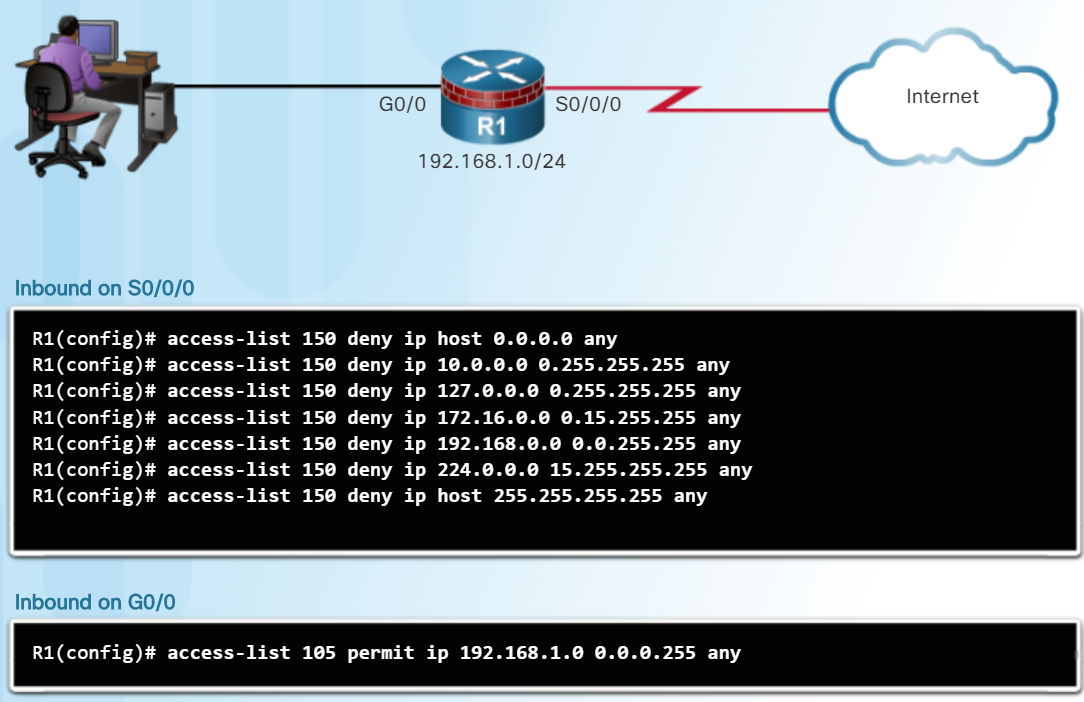
\includegraphics[width=10\xm]{pictures/AntispoofingACL.PNG}
  \end{figure}

Hackers can use ICMP echo packets (pings) to discover network, generate DoS flood attacks, or alter host routing tables. Both ICMP echo and redirect messages should be blocked \emph{inbound} by the router. Several ICMP messages are recommended for proper network operation and should be allowed into the internal network:

\begin{itemize}
\item Echo reply -- Allows users to ping external hosts.
\item Source quench -- Requests that the sender decrease the traffic rate of messages.
\item Unreachable -- Generated for packets that are administratively denied by an ACL.
\end{itemize}

Several ICMP messages are required for proper network operation and should be allowed to exit the network (outbound ACL):

\begin{itemize}
\item Echo -- Allows users to ping external hosts.
\item Parameter problem -- Informs the host of packet header problems.
\item Packet too big -- Enables packet maximum transmission unit (MTU) discovery.
\item Source quench -- Throttles down traffic when necessary.
\end{itemize}

As a rule, block all \emph{other} ICMP message types \emph{outbound}.\\

If SNMP is necessary, exploitation of SNMP vulnerabilities can be mitigated by applying interface ACLs to filter SNMP packets from non-authorized systems.  The most effective means of exploitation prevention is to disable the SNMP server on IOS devices for which it is not required. 

\note See also \emph{CCNA notebook} for ACL configuration and IPv6 ACL.

\section{Firewall}

All firewalls share some common properties: resistant to attacks, the only transit point between networks because all traffic flows through the firewall, enforce the access control policy. There are two configuration models for Cisco IOS Firewall: \hyperref[sec:ClassicFirewall]{Classic Firewall} and \hyperref[sec:ZPF]{Zone-based Policy Firewall (ZPF)}.\\

\subsection{Packet filtering}

Basic packet filtering firewalls can only filter based on Layer 3 and sometimes basic Layer 4 information. 

\textbf{Benefits:} Simple implementation, Low impact on network performance, Initial degree of security at the network layer, Almost all the tasks of a high-end firewall at a much lower cost.\\

\textbf{Limitations:} Susceptible to IP spoofing, Not reliably filter fragmented packets, Complex ACLs (difficult to implement and maintain), \emph{Stateless:} examine each packet individually rather than in the context of the state of a connection.

\subsection{Statefull firewall}

Stateful firewall monitors network traffic as it flows into and out of the organization and determines whether packets belong to an existing connection or are from an unauthorized source. Stateful filtering tracks each connection and confirms that they are valid. Stateful firewalls use a state table to keep track of the actual communication process.\\ 

\textbf{Benefits:} prevent spoofing and DoS attacks, provide more stringent control over security.\\ 

\textbf{Limitations:} cannot prevent Application Layer attacks, does not filter UDP and ICMP packets, cannot track connections that use dynamic port negotiation, not support authentication.

\subsection{Next-Generation Firewall}

Designed with advanced malware protection, the Cisco ASA with FirePOWER services is also called the \textbf{Cisco ASA Next-Generation Firewall} because it is an adaptive, threat-focused firewall. It is designed to provide defense across the entire attack continuum, which includes before, during, and after attacks.

\subsection{DMZ}

A demilitarized zone (DMZ) is a firewall design where there is typically one inside interface connected to the private network, one outside interface connected to the public network, and one DMZ interface, as shown in the figure \ref{DMZfilter}.

\begin{figure}[hbtp]
\caption{DMZ topology and traffic restriction}\label{DMZfilter}
\centering
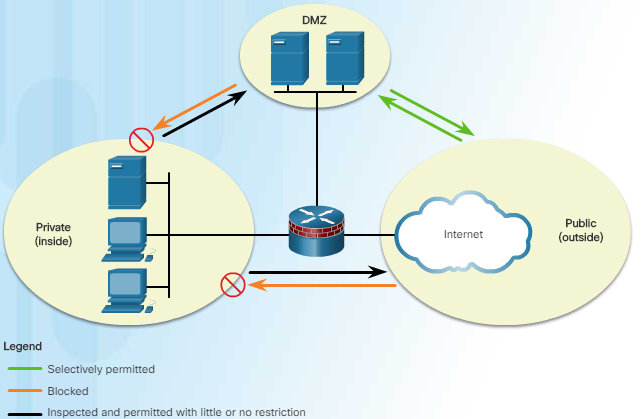
\includegraphics[width=10\xm]{pictures/DMZfilter.PNG}
\end{figure}

\begin{itemize}
\item Private network $\rightarrow$ DMZ: Inspected 
\item DMZ  $\rightarrow$ Private network: Blocked
\item Public network  $\leftrightarrow$ DMZ: selectively permitted
\item Private network $\rightarrow$ Public network: Inspected
\item Public network $\rightarrow$ Private network: Blocked
\end{itemize}

\subsection{Layered Defense}

A layered defense uses different types of firewalls that are combined in layers. Security policies can be enforced between the layers and inside the layers. A traffic from the untrusted network has to go through the following layers and policies:

\begin{enumerate}
\item Edge router (packet filtering)
\item Bastion host (hardened computer located in the DMZ\footnote{This type of DMZ setup is called a \emph{screened subnet configuration}.}) or Screened firewall
\item Interior screening router
\end{enumerate}

\subsection{Classic firewall}\label{sec:ClassicFirewall}

Classic Firewall (CBAC) is a \emph{stateful} firewall that provides four main functions: Filtering, Inspection, Intrusion detection, and Generation of audits and alerts. It can only detects and protects against external attacks.\\ 

Classic Firewall creates \emph{temporary} openings in the ACL to allow returning traffic. These entries are created as inspected traffic leaves the network and are removed when the connection terminates or the idle timeout period for the connection is reached. 
In addition to extended ACLs, Application layer protocol session information is used by a classic firewall to filter traffic. Figure \ref{ClassicFirewall} shows how Classic Firewall inspects SSH traffic.

\begin{figure}[hbtp]
\caption{Classic Firewall inspects SSH traffic}\label{ClassicFirewall}
\centering
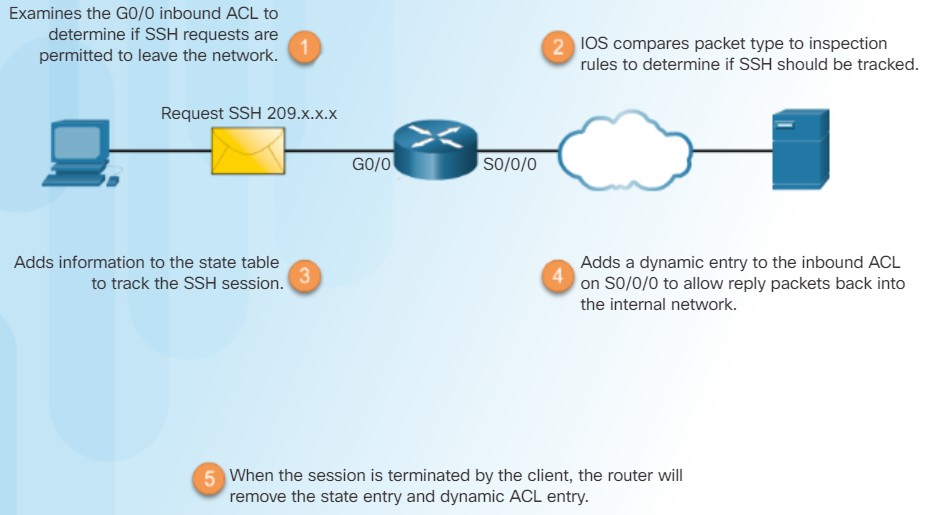
\includegraphics[ width=10\xm ]{pictures/ClassicFirewall.PNG}
\end{figure}

Take the topology in figure \ref{ClassicConfig} as an example for configuration. Suppose that the administrator wants to allow SSH sessions between the 10.0.0.0 and 172.30.0.0 networks. However, only hosts from the 10.0.0.0 network are allowed to initiate SSH sessions. All other access is denied. 

\begin{figure}[hbtp]
\caption{Network topology}\label{ClassicConfig}
\centering
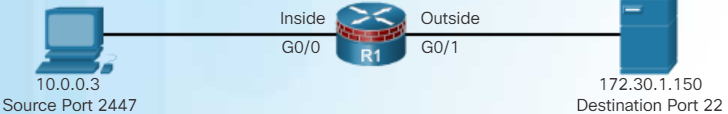
\includegraphics[width=10\xm]{pictures/ClassicConfig.PNG}
\end{figure}


\begin{sexylisting}{Classic Firewall configuration}
ip access-list extended INSIDE
  permit tcp 10.0.0.0 0.0.0.255 any eq 22
ip access-list extended OUTSIDE
  deny ip any any

ip inspect name FWRULE ssh

interface g0/0
  ip access-group INSIDE in
  ip inspect FWRULE in
interface g0/1
  ip access-group OUTSIDE in
\end{sexylisting}

There are four steps to configure this policy using a Classic Firewall:

\begin{enumerate}
\item \textbf{Define the internal and external interfaces}: G0/0 is the inside interface and G0/1 is the outside interface.
\item \textbf{Configure ACLs for each interface}: The INSIDE ACL allows only SSH traffic from the 10.0.0.0 network; the OUTSIDE ACL will deny inbound traffic from the 172.30.0.0 network.
\item \textbf{Define inspection rules}: The inspection rule FWRULE specifies that traffic will be inspected for SSH connections. This inspection rule has no effect until it is applied to an interface.
\item \textbf{Apply an inspection rule to an interface}: When the FWRULE is applied to inbound traffic on the G0/0 interface, the Classic Firewall configuration will dynamically add an entry to allow inbound SSH traffic from the 172.30.0.0 network. From now on, the FWRULE inspects SSH traffic between 10.0.0.0 and 172.30.0.0 network.
\item \textbf{Verification}: Use \code{show ip inspect sessions} command to verify inspect sessions.
\end{enumerate}

\subsection{Zone-based Policy Firewall (ZPF)}\label{sec:ZPF}

The Classic Firewall applies firewall policy to interfaces. Zone-Based Policy Firewall uses zones to apply firewall policy.\\

ZPFs use the concept of zones to provide additional flexibility. A zone is a group of one or more interfaces that have similar functions or features. By default, the traffic between interfaces in the same zone is not subject to any policy and passes freely. However, all zone-to-zone traffic is blocked. In order to permit traffic between zones, a policy allowing or inspecting traffic must be configured.\\

There are several benefits of a ZPF:

\begin{itemize}
\item Not dependent on ACLs.
\item The router security posture is to block unless explicitly allowed.
\item Policies are easy to read and troubleshoot with the Cisco Common Classification Policy Language (C3PL). C3PL can create traffic policies based on events and affect any given traffic with only one policy, instead of needing multiple ACLs and inspection actions.
\end{itemize}

There are three possible actions with Cisco IOS Zone-Based Policy Firewall:

\begin{itemize}
  \item The inspect action configures Cisco IOS stateful packet inspection.
  \item The drop action is similar to a deny ACE.
  \item The pass action is similar to a permit ACE but does not track the state of connections or sessions.​
\end{itemize}

ZPF Rules for Transit Traffic between two interfaces depends on the zone that those interfaces belongs to:

\begin{itemize}
\item Neither intefaces is a zone member: Pass
\item Both interfaces are members of the same zone: Pass
\item Interfaces belong to different zones: Action defined by policy
\item Only one interface is a zone member: Drop
\end{itemize}

The \emph{self zone} is a special zone which is the router itself and includes all the router interface IP addresses. By default, if the router (self zone) is the source or the destination, then all traffic is permitted. The only exception is if the source and destination are a zone-pair with a specific service-policy. In that case, the policy is applied to all traffic.

There are four steps to configure a ZPF zone (Take the topology in figure \ref{Zone} as an example):

\begin{enumerate}
\item \textbf{Create the zones and Assign zones to appropriate interfaces:} Associating a zone to an interface will immediately apply the service-policy that has been associated with the zone. If no service-policy is yet configured for the zone, all transit traffic will be dropped. Use the \code{zone-member security} command to assign a zone to an interface. In the example, g0/1 is assigned the PRIVATE zone, and s0/0/0 is assigned the INTERNET zone, and g0/0 is assigned to DMZ zone.

\item \textbf{Identify traffic with class-map:} A class is a way of identifying a set of packets based on its contents using \code{match} conditions. Packets must meet one of the match criteria \code{match-any} or all of the match criteria \code{match-all} to be considered a member of the class. Table \ref{tab:classMap} shows the syntax for the \code{class-map} and its sub-commands.

\item \textbf{Define an action with policy-map:} Assign class-maps (PRIVATE-ACL-CLASS and PRIVATE-INTERNET-CLASS) to a policy-map and define what action (Inspect, Drop, or Pass) should be taken for traffic that is a member of a class. 
\item \textbf{Identify a zone-pair and match it to a policy-map:} The example commands below create a zone pair PRIVATE-2-INTERNET between PRIVATE and INTERNET, and associate that zone pair to a policy-map PRIV-TO-PUB-POLICY.
\end{enumerate}

\begin{figure}[hbtp]
\caption{ZPF configuration topology}\label{Zone}
\centering
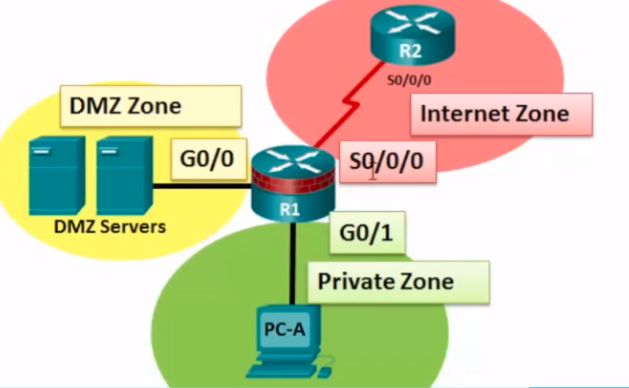
\includegraphics[scale=0.5]{pictures/Zone.PNG}
\end{figure}

\begin{sexylisting}{ZPF configuration}
#STEP 1
zone security PRIVATE
zone security INTERNET
zone security DMZ
int g0/1
  zone-member security PRIVATE
int s0/0/0
  zone-member security INTERNET    
int g0/0
  zone-member security DMZ
exit

#STEP 2
class-map type inspect match-all PRIVATE-ACL-CLASS
  match access-group 100    
class-map type inspect match-any PRIVATE-INTERNET-CLASS
  match protocol http
  match protocol https
  match protocol dns
exit    

#STEP 3
policy-map type inspect PRIV-TO-PUB-POLICY
  class type inspect PRIVATE-ACL-CLASS   
  inspect    
  class type inspect PRIVATE-INTERNET-CLASS
  inspect
  class class-default
exit   

#STEP 4
zone-pair security PRIVATE-2-INTERNET source PRIVATE destination INTERNET
  service-policy type inspect  PRIV-TO-PUB-POLICY
end
\end{sexylisting}

\tableStart[\caption{The syntax of class-map command}\label{tab:classMap}] { |p{5\xm}|p{8\xm}| }
\multicolumn{2}{|c|}{ \code{class-map type inspect [match-any | match-all] <class-name>} } \w
\head{Parameter}&\head{Description} \w
\code{match-any} & Packets must meet one of the criteria to be considered a member of the class.\w
\code{match-all} & Packets must meet all of the criteria to be considered a member of the class.\w
\code{match protocol <protocol-name>} & Configure criteria based on specified protocol.\w
\code{match access-group <acl-name>} & Configure criteria based on specified ACL.\w
\code{match class-map <class-name>} & Use another class-map as criteria.\w
\tableEnd

\begin{itemize}
\item \code{inspect} -- This action offers state-based traffic control. It tracks UDP or TCP connections and permit the return traffic.
\item \code{drop} -- This is the default action for all traffic. Similar to the implicit deny any at the end of every ACL, , there is an explicit \code{drop} applied to the end of every policy-map.
\item \code{pass} -- This action allows \emph{one-direction} traffic between two zones, and does not track the state of connections. A corresponding policy must be applied to allow return traffic to pass in the opposite direction. This action is ideal for secure protocols, such as IPsec. 
\end{itemize}

The fourth step is to identify a zone pair (\\

\begin{sexylisting}{ZPF Verification}
show run | begin class-map
show run | begin class-map
show class-map type inspect
show zone security
show zone-pair security
show policy-map type inspect
show policy-map type inspect zone-pair sessions
\end{sexylisting}

The service-policy is now active. HTTP, HTTPS, and DNS traffic sourced from the PRIVATE zone and destined for the PUBLIC zone will be inspected. Traffic sourced from the PUBLIC zone and destined for the PRIVATE zone will only be allowed if it is part of sessions originally initiated by PRIVATE zone hosts.

\subsection{ZPF Configuration Considerations}

\begin{itemize}
\item The router never filters the traffic between interfaces in the same zone.
\item An interface cannot belong to multiple zones.
ZPF can coexist with Classic Firewall although they cannot be used on the same interface. Remove the \code{ip inspect} interface configuration command before applying the \code{zone-member security} command.
\item Traffic can never flow between an interface assigned to a zone and an interface without a zone assignment. Applying the zone-member configuration command always results in a temporary interruption of service until the other zone-member is configured.
\item Communication between zones are, by default, dropped. Unless there exits a service-policy configured for the zone-pair.
\item The \code{zone-member} command does not protect the router itself (traffic to and from the router is not affected) unless the zone-pairs are configured using the predefined self zone.
\end{itemize}